% Options for packages loaded elsewhere
\PassOptionsToPackage{unicode}{hyperref}
\PassOptionsToPackage{hyphens}{url}
%
\documentclass[
]{article}
\usepackage{lmodern}
\usepackage{amssymb,amsmath}
\usepackage{ifxetex,ifluatex}
\ifnum 0\ifxetex 1\fi\ifluatex 1\fi=0 % if pdftex
  \usepackage[T1]{fontenc}
  \usepackage[utf8]{inputenc}
  \usepackage{textcomp} % provide euro and other symbols
\else % if luatex or xetex
  \usepackage{unicode-math}
  \defaultfontfeatures{Scale=MatchLowercase}
  \defaultfontfeatures[\rmfamily]{Ligatures=TeX,Scale=1}
\fi
% Use upquote if available, for straight quotes in verbatim environments
\IfFileExists{upquote.sty}{\usepackage{upquote}}{}
\IfFileExists{microtype.sty}{% use microtype if available
  \usepackage[]{microtype}
  \UseMicrotypeSet[protrusion]{basicmath} % disable protrusion for tt fonts
}{}
\makeatletter
\@ifundefined{KOMAClassName}{% if non-KOMA class
  \IfFileExists{parskip.sty}{%
    \usepackage{parskip}
  }{% else
    \setlength{\parindent}{0pt}
    \setlength{\parskip}{6pt plus 2pt minus 1pt}}
}{% if KOMA class
  \KOMAoptions{parskip=half}}
\makeatother
\usepackage{xcolor}
\IfFileExists{xurl.sty}{\usepackage{xurl}}{} % add URL line breaks if available
\IfFileExists{bookmark.sty}{\usepackage{bookmark}}{\usepackage{hyperref}}
\hypersetup{
  pdftitle={space\{3in\}BDA - Project},
  pdfauthor={Tomi Räsänen - 879626 \& Erik Husgafvel - 528867},
  hidelinks,
  pdfcreator={LaTeX via pandoc}}
\urlstyle{same} % disable monospaced font for URLs
\usepackage[margin=1in]{geometry}
\usepackage{color}
\usepackage{fancyvrb}
\newcommand{\VerbBar}{|}
\newcommand{\VERB}{\Verb[commandchars=\\\{\}]}
\DefineVerbatimEnvironment{Highlighting}{Verbatim}{commandchars=\\\{\}}
% Add ',fontsize=\small' for more characters per line
\usepackage{framed}
\definecolor{shadecolor}{RGB}{248,248,248}
\newenvironment{Shaded}{\begin{snugshade}}{\end{snugshade}}
\newcommand{\AlertTok}[1]{\textcolor[rgb]{0.94,0.16,0.16}{#1}}
\newcommand{\AnnotationTok}[1]{\textcolor[rgb]{0.56,0.35,0.01}{\textbf{\textit{#1}}}}
\newcommand{\AttributeTok}[1]{\textcolor[rgb]{0.77,0.63,0.00}{#1}}
\newcommand{\BaseNTok}[1]{\textcolor[rgb]{0.00,0.00,0.81}{#1}}
\newcommand{\BuiltInTok}[1]{#1}
\newcommand{\CharTok}[1]{\textcolor[rgb]{0.31,0.60,0.02}{#1}}
\newcommand{\CommentTok}[1]{\textcolor[rgb]{0.56,0.35,0.01}{\textit{#1}}}
\newcommand{\CommentVarTok}[1]{\textcolor[rgb]{0.56,0.35,0.01}{\textbf{\textit{#1}}}}
\newcommand{\ConstantTok}[1]{\textcolor[rgb]{0.00,0.00,0.00}{#1}}
\newcommand{\ControlFlowTok}[1]{\textcolor[rgb]{0.13,0.29,0.53}{\textbf{#1}}}
\newcommand{\DataTypeTok}[1]{\textcolor[rgb]{0.13,0.29,0.53}{#1}}
\newcommand{\DecValTok}[1]{\textcolor[rgb]{0.00,0.00,0.81}{#1}}
\newcommand{\DocumentationTok}[1]{\textcolor[rgb]{0.56,0.35,0.01}{\textbf{\textit{#1}}}}
\newcommand{\ErrorTok}[1]{\textcolor[rgb]{0.64,0.00,0.00}{\textbf{#1}}}
\newcommand{\ExtensionTok}[1]{#1}
\newcommand{\FloatTok}[1]{\textcolor[rgb]{0.00,0.00,0.81}{#1}}
\newcommand{\FunctionTok}[1]{\textcolor[rgb]{0.00,0.00,0.00}{#1}}
\newcommand{\ImportTok}[1]{#1}
\newcommand{\InformationTok}[1]{\textcolor[rgb]{0.56,0.35,0.01}{\textbf{\textit{#1}}}}
\newcommand{\KeywordTok}[1]{\textcolor[rgb]{0.13,0.29,0.53}{\textbf{#1}}}
\newcommand{\NormalTok}[1]{#1}
\newcommand{\OperatorTok}[1]{\textcolor[rgb]{0.81,0.36,0.00}{\textbf{#1}}}
\newcommand{\OtherTok}[1]{\textcolor[rgb]{0.56,0.35,0.01}{#1}}
\newcommand{\PreprocessorTok}[1]{\textcolor[rgb]{0.56,0.35,0.01}{\textit{#1}}}
\newcommand{\RegionMarkerTok}[1]{#1}
\newcommand{\SpecialCharTok}[1]{\textcolor[rgb]{0.00,0.00,0.00}{#1}}
\newcommand{\SpecialStringTok}[1]{\textcolor[rgb]{0.31,0.60,0.02}{#1}}
\newcommand{\StringTok}[1]{\textcolor[rgb]{0.31,0.60,0.02}{#1}}
\newcommand{\VariableTok}[1]{\textcolor[rgb]{0.00,0.00,0.00}{#1}}
\newcommand{\VerbatimStringTok}[1]{\textcolor[rgb]{0.31,0.60,0.02}{#1}}
\newcommand{\WarningTok}[1]{\textcolor[rgb]{0.56,0.35,0.01}{\textbf{\textit{#1}}}}
\usepackage{graphicx}
\makeatletter
\def\maxwidth{\ifdim\Gin@nat@width>\linewidth\linewidth\else\Gin@nat@width\fi}
\def\maxheight{\ifdim\Gin@nat@height>\textheight\textheight\else\Gin@nat@height\fi}
\makeatother
% Scale images if necessary, so that they will not overflow the page
% margins by default, and it is still possible to overwrite the defaults
% using explicit options in \includegraphics[width, height, ...]{}
\setkeys{Gin}{width=\maxwidth,height=\maxheight,keepaspectratio}
% Set default figure placement to htbp
\makeatletter
\def\fps@figure{htbp}
\makeatother
\setlength{\emergencystretch}{3em} % prevent overfull lines
\providecommand{\tightlist}{%
  \setlength{\itemsep}{0pt}\setlength{\parskip}{0pt}}
\setcounter{secnumdepth}{-\maxdimen} % remove section numbering
\usepackage{amsmath}

\title{space\{3in\}BDA - Project}
\author{Tomi Räsänen - 879626 \& Erik Husgafvel - 528867}
\date{}

\begin{document}
\maketitle

\newpage

{
\setcounter{tocdepth}{2}
\tableofcontents
}
\newpage

\hypertarget{introduction}{%
\section{1. Introduction}\label{introduction}}

One of the biggest challenges of humankind in the 2020s is figuring out
ways to slow down the growth of greenhouse gas emissions and stop global
warming (due to human activities) under 2 \(^{\circ}\)C. The increasing
trend of global temperature is easily seen in Figure
\ref{fig:global_temp} {[}cite NASA{]} in which the global surface
temperature is illustrated relative to 1951-1980 average temperatures.
Warming can also be seen with one's own eyes by observing the winters
that are warming year by year, by noticing that the number of
devastating hurricanes is increased, and by finding out the increased
rate of ice melting in glaciers during summer.

\begin{figure}
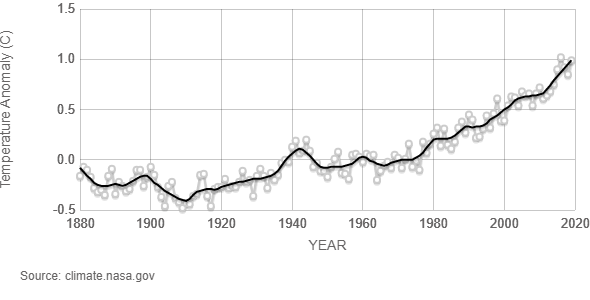
\includegraphics[width=1\linewidth]{GlobalTemp} \caption{\label{fig:global_temp}Global Land-Ocean Temperature Index}\label{fig:globaltemp}
\end{figure}

In response to that warming, many countries have declared a climate
emergency to emphasize the criticality of the situation. In addition,
young people have organized climate demonstrations around the world,
politicians are talking more and more about climate change, and
presidents and prime ministers are negotiating agreements and
commitments to solve this, one of humanity's greatest, problem. But what
if, despite attempts of negotiation, the necessary CO\(_2\) reduction
decisions are not achieved?

In this project, our goal is to model the historical emission trends of
selected countries as well as attempts to model their future emissions.
We are examining a scenario in which emissions continue to develop at a
historical rate, and the necessary reductions are not achieved. In our
modeling, the other parameters e.g.~population growth and technical
conditions, are similar to historical data in our modeling.

\hypertarget{data-description}{%
\section{2. Data description}\label{data-description}}

Our CO\(_2\) data was obtained from \textit{Our World in Data} (OWID)
web page {[}cite OWID\_net{]} and the actual \textit{CSV} file from OWID
GitHub page {[}cite OWID\_git{]}. As mentioned earlier, climate change
is a hot topic in the daily news, and there is a lot of studies and
research concerning how CO\(_2\) emissions are influencing global
warming. The data set was also used, for example, when researchers
studied the climate impact of the different policy recommendation which
targeted to reduce greenhouse gases from the atmosphere.

\hypertarget{choosing-the-sample-and-estimating-its-resemblance}{%
\subsection{2.1 Choosing the sample and estimating it's
resemblance}\label{choosing-the-sample-and-estimating-its-resemblance}}

In our modeling, we selected 19 different countries from the OWID data
set and examined CO\(_2\) data between the years 1950-2018. We decided
to not take all countries into the modeling as the are holes and missing
information in the dataset. The countries we chose cover the whole globe
and are roughly evenly distributed across continents. However, we
estimated that the data is probably more reliable in the western
countries and thus were more open-minded in selecting them. Even that
said, we think that the geographical distribution covers the whole world
pretty well. Another important aspect of division is the division
between large and small emitters. Even though it is quite difficult to
perform such division, we tried to take countries from both ends pretty
evenly. However, it is worth noting that this division was performed
intuitively and it does not rely on any actual metrics. Lastly, we
thought that the division between developing and western countries is
extremely important to consider too. Therefore, this aspect was taken
into account when considering the sample countries, too. We estimated
that the number of developing countries in the world exceeds the number
of western countries and thus tried to choose developing countries a bit
more into the sample set.

For the reasons presented above, we believe that the sample we use in
this project, resembles the situation in the world quite well. However,
we estimated that it is possible that the sample is slightly biased
towards western countries. It is important to note this since we examine
results where the CO2-emissions data is standardized with the countries'
population. As the CO2-emissions are standardized, the importance of
correct ratio (number) of countries between different division-aspects
increases. As the sample may be a bit biased, the results may propose
higher numbers of CO2-emissions per capita in the world than what they
actually are.

\hypertarget{plotting-the-sample}{%
\subsection{2.2 Plotting the sample}\label{plotting-the-sample}}

Below is plotted three graphs. On the first row, we investigate our
sample countries' CO2-emissions by country. Please note the y-axis
difference between large and small emitters in the graphs. It is worth
noting that the CO2-emissions development of China is very concerning as
it has almost doubled its CO2-emissions during the last 15 years. In
addition, India, Greece, Morocco, Peru and Mongolia has been showing a
bit concerning trend during last decades.

On the second row, we plotted the sample countries' emission
standardized with the population of the country. Thus, we obtained a
``CO2 per capita'' -estimate for each country. This is the data that we
used later in our models. Especially between 1950s and 70s, western
countries play significant role as the big emitters. However, during
2000s, the situation has changed as western countries have
systematically been able to lower their emissions per capita. At the
same time, developing countries have been increasing their emissions and
thus the situation has tied.

\begin{center}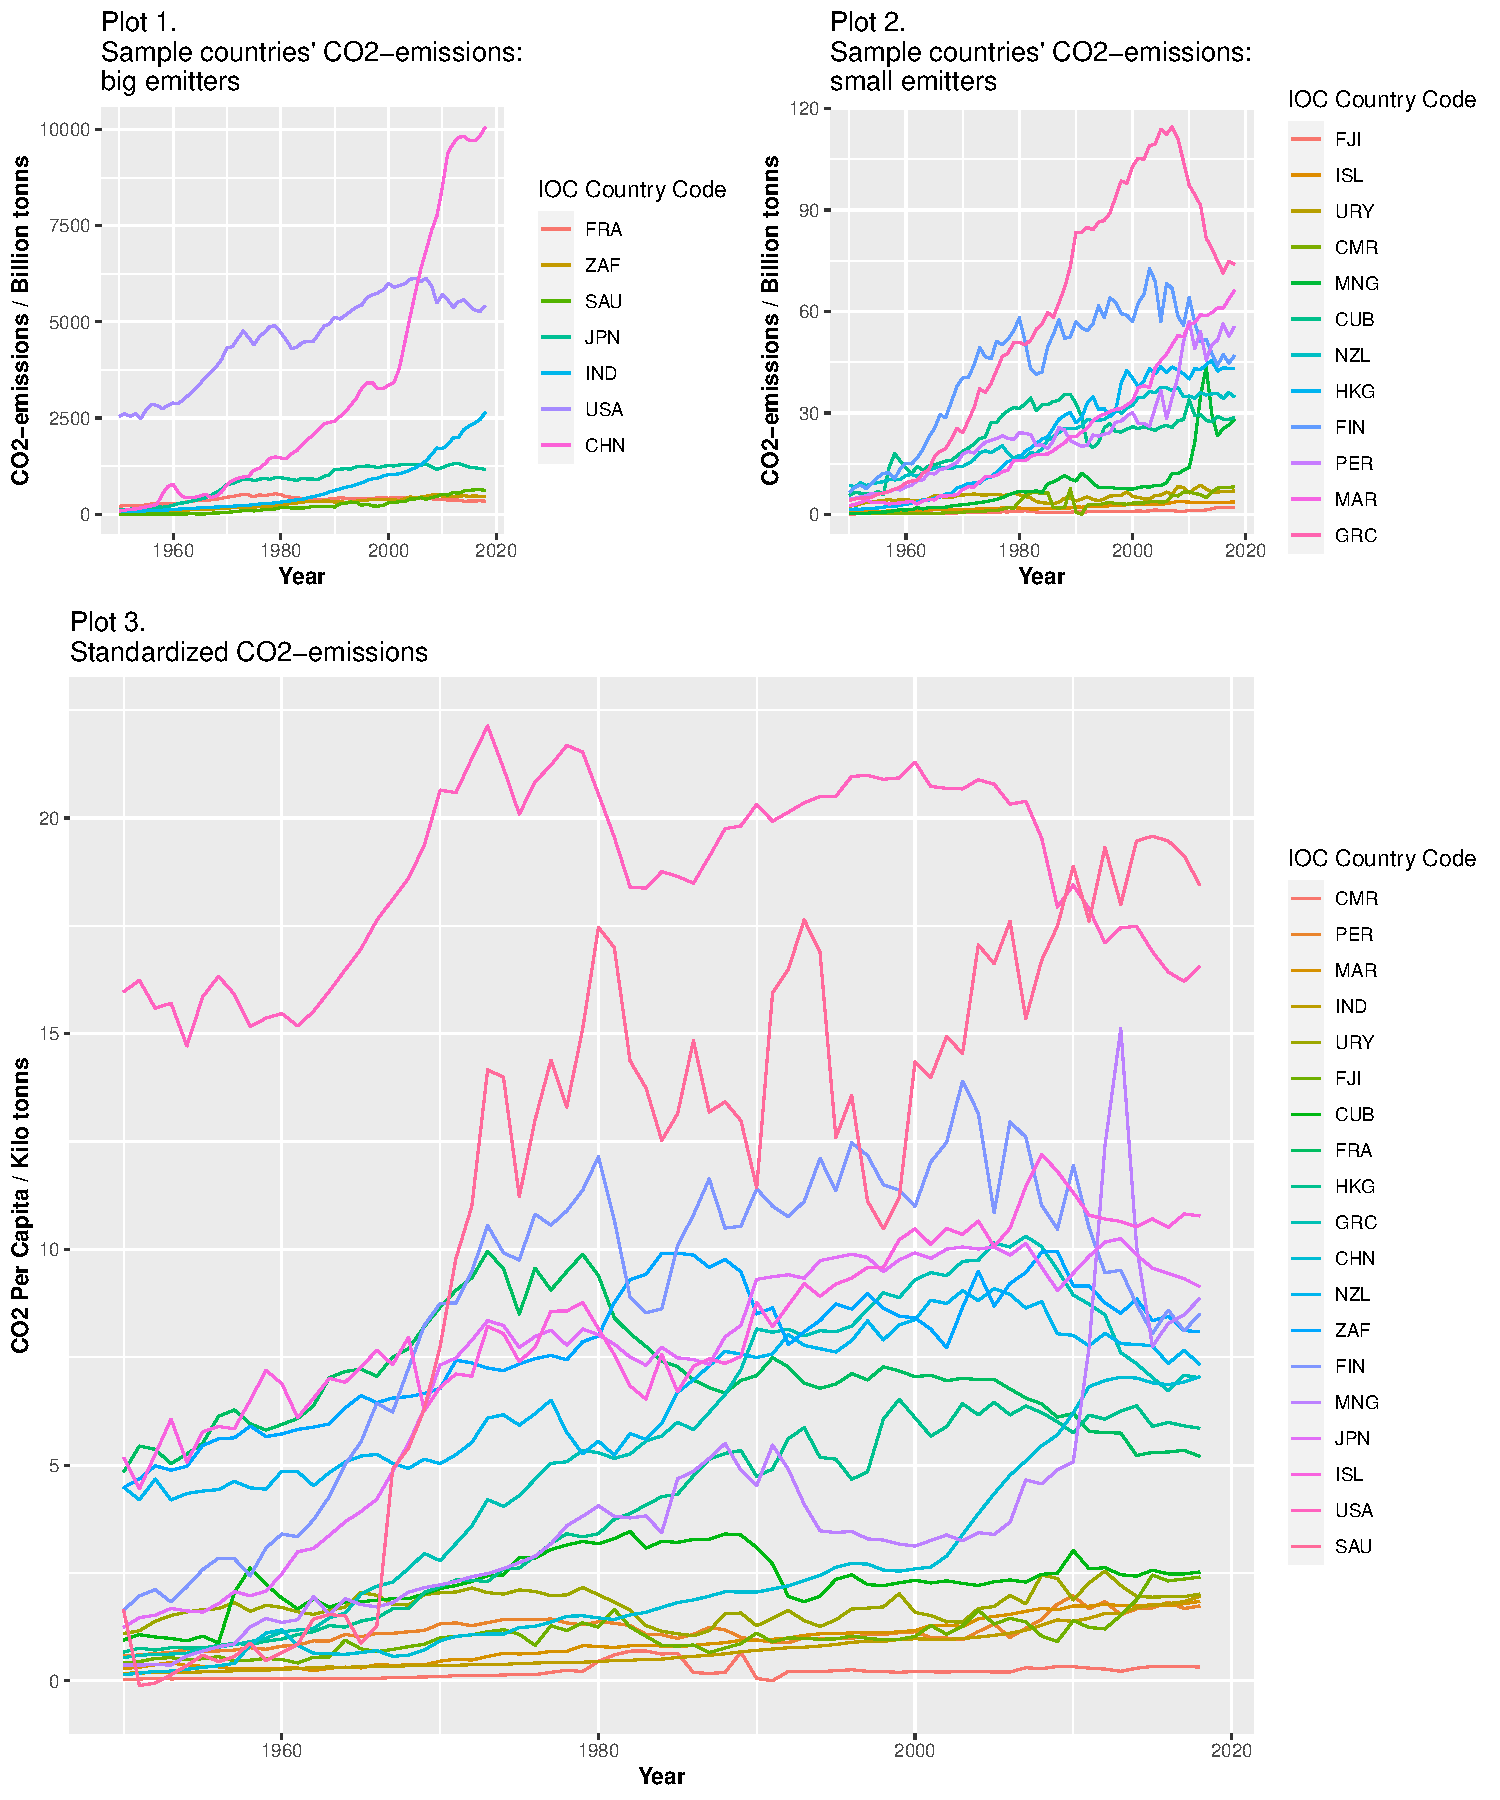
\includegraphics{project_files/figure-latex/fig1-1} \end{center}

\hypertarget{model-description}{%
\section{3 Model description}\label{model-description}}

In this chapter, we will present our model structures and stan codes of
our implementation of a non-hierarchical pooled model and a hierarchical
model. Before this, we briefly introduce the mathematical structure
behind the models.

\hypertarget{pooled-model}{%
\subsection{3.1 Pooled model}\label{pooled-model}}

A pooled model is one of the most straightforward model structure to
understand. In the pooled model, all data points are used as one
``pool'' without considering groups or particular features different
pieces of data could have. The whole dataset is used as a one, and
modeling is done based on that collection of data. If we assume that
priors of the mean and standard deviation follow standard normal
distributions, we can present the mathematical structure of the pooled
model in the form

\begin{align}\label{eq1}
     \mu & \sim N(0,1) \\
     \sigma & \sim N(0,1) \\
     y_i & \sim N(\mu,\sigma)
\end{align}

We used these standardized normal priors just for illustration purposes,
and the correct choice of priors we utilized when modeling is presented
in chapter 4. Respectively, the pooled model's implementation with
probabilistic programming language \emph{Stan} is presented in chapter
5.

\hypertarget{hierarchical-normal-model}{%
\subsection{3.2 Hierarchical normal
model}\label{hierarchical-normal-model}}

Unlike the previous model, the hierarchical model takes into account the
possibility that some of the subgroups of the whole dataset have similar
properties. Due to this observation, the hierarchical model presents a
``hyper-prior'' that is common to each group. For each group, its
posterior distribution of mean is calculated using that hyper-prior,
taking into account only all samples belonging to that group. This
property can be illustrated in Figure \ref{fig:hier_sketch}. In Figure
\ref{fig:hier_sketch}, \(\tau\) is a hyper-parameter and \(\theta_i\)s
presents modeled parameter of each group.

\begin{figure}
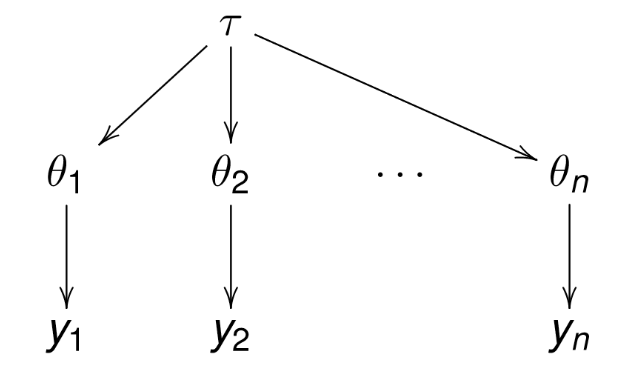
\includegraphics[width=1\linewidth]{hier_model} \caption{\label{fig:hier_sketch}A hierarchical model -- }\label{fig:hier}
\end{figure}

We can summarize the hierarchical model mathematically as

\begin{align}\label{eq2}
     \mu_0 & \sim N(0,1) \\
     \sigma_0 & \sim N(0,1) \\
     \mu_i & \sim N(\mu_0, \sigma_0) \\
     \sigma & \sim N(0,1) \\
     y_{ji} & \sim N(\mu_i,\sigma)
\end{align}

where \(mu_0\) and \(sigma_0\) are hyper-priors for mean and standard
deviation. Again, we used these normal distributions just for
illustration purposes. In addition, we assumed through the project that
all the groups have a common variance (\(\sigma\) in {[}\ref{eq2}{]}).

\hypertarget{priors}{%
\section{4. Priors}\label{priors}}

For our modeling, we needed to define hyper priors \(\mu_0\) and
\(\sigma_0\). In addition, common \(\sigma\) was defined for the
hierarchical model's standard deviation between data points.

Our first goal was to define the hyper prior \(\mu_0\). To aid this
problem, we searched information in the internet about country-wise
CO2-emissions per capita. The figure below illustrates the results that
we found. The figure is taken from
\url{https://www.economicshelp.org/blog/10296/economics/top-co2-polluters-highest-per-capita/}
on the 1st of December, 2020.

\begin{figure}
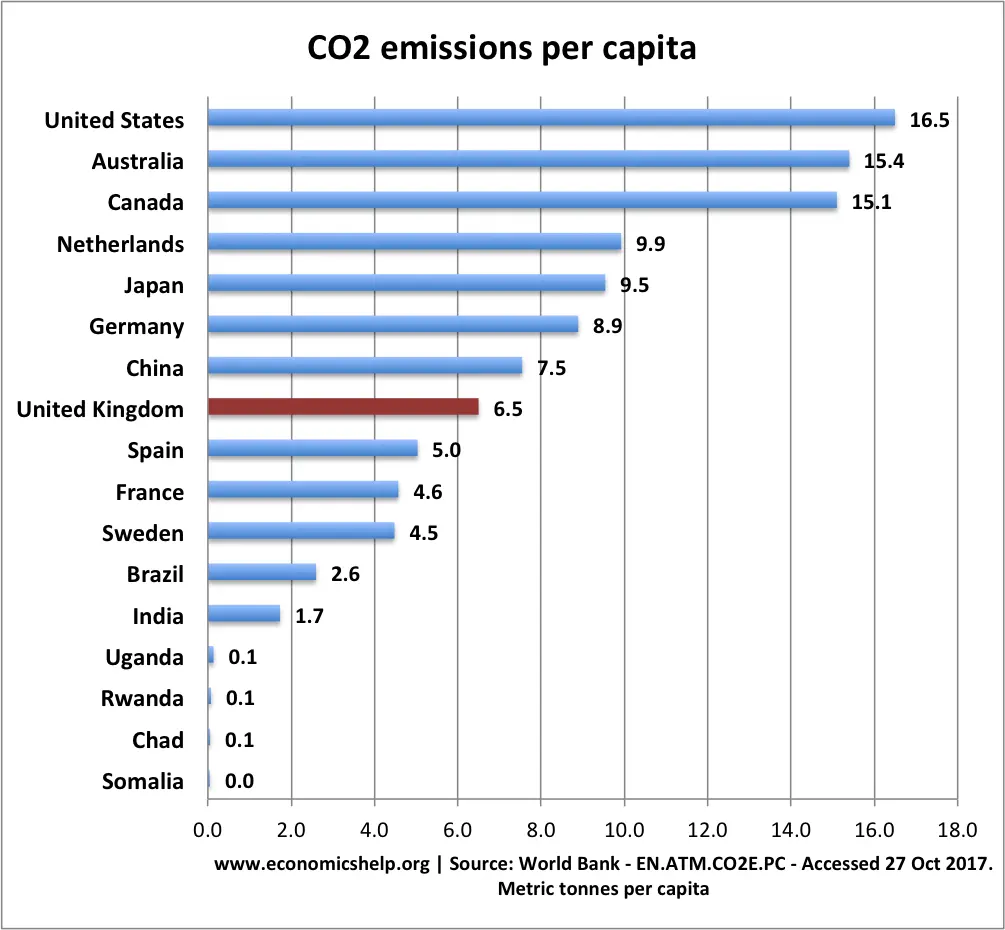
\includegraphics[width=1\linewidth]{co2-emissions-per-capita} \caption{\label{fig:co2-emissions-per-capita}Selected countries CO2 emissions per capita \newline Source: https://www.economicshelp.org/blog/10296/economics/top-co2-polluters-highest-per-capita/ \newline Accessed December 1, 2020.}\label{fig:co2-emissions-per-capit}
\end{figure}

Results shown in the Figure \ref{fig:co2-emissions-per-capita} represent
selected countries on year 2016 and are pretty well aligned with the
CO2-emissions per capita that we calculated and drew at our data
description section. However, it seems that the underlying dataset is
not the same that we decided to use in this project. The idea of
searching external information from the internet is to obtain a better
understanding about the underlying truth without having to use our own
dataset at this point. We want to emphasize that at this point we used
our dataset only to estimate whether our own dataset is aligned with the
other information found from the internet or not aligned at all.

\hypertarget{choosing-hyper-prior-mu}{%
\subsection{4.1 Choosing hyper prior mu}\label{choosing-hyper-prior-mu}}

With the information that we obtained from investigating the internet
more thoroughly, we were able to estimate the order of magnitude for the
CO2-emissions per capita. Considering our range of fluctuation, we can
first exclude the results below zero. There won't be negative values in
CO2-emissions calculations. On the other end, we estimated that the
values won't exceed 50 kilo tonns per year per country. However, given
the information that we were able to obtain, we believe that there is a
lot of space for error in value range {[}0,50{]}. Thus, we believe that
the actual expected mean for hyper prior \(\mu_0\) is closer to 0 than
50. We estimated that most of the values should be somewhere between 0
and 30. Therefore, the expected value for \(\mu_0\) was placed to 15:
\(E(\mu_0) = 15\). With the observations presented above, we were
finally able to estimate the distribution for \(\mu_0\):
\(\mu_0 \sim logN(2.58, 0.5)\) seems to be reasonable. With this
distribution and values, \(\mu_0\) is strictly restricted to the
positive values, has it's expected value \(E(\mu_0) \approx 15.0\) and
the \(P(\mu_0 < 50) \approx 1.00\).

\hypertarget{choosing-hyper-prior-sigma}{%
\subsection{4.2 Choosing hyper prior
sigma}\label{choosing-hyper-prior-sigma}}

Next, we had to consider the distribution for the hyper prior
\(\sigma_0\). Again, restricting the values to positive side only seems
reasonable. In our consideration, we prioritized that the probability
for \(\sigma_0\) being zero would be low but on the contrary, the values
close to zero would have high probability. Estimating the appropriate
tail for the distribution was rather difficult with the information that
we were able to obtain. Therefore, we used iterative method to find
suitable hyper prior \(\sigma_0\). We ended up to a Gamma distribution
\(Gamma(\alpha = 2.5,\beta = 0.8)\). This distribution gives
\(E(\sigma_0) = 1\) and \(P(\sigma_0 < 6) \approx 0.99\). This seems
reasonable, as we do not want to narrow the \(\mu_j\) distributions too
much with our prior choices.

\hypertarget{choosing-common-sigma-for-observations}{%
\subsection{4.3 Choosing common sigma for
observations}\label{choosing-common-sigma-for-observations}}

Choosing the common sigma for given data points (observations), one can
try to answer to a question, how big a jump could the data make between
observations n and n+1. Given our relatively small value range
{[}0,50{]} and a fact that the data observations derive from countries'
CO2-emissions per capita, we consider the jumps to be only some unit
digits at most. For example, with standard deviation of 2, the
probability that the ``random'' jump from n to n+1 being greater than 2
is roughly 0.3, which is relatively big probability for such a big jump
given circumstances. We believe that the changes within country
CO2-emissions per capita tend to be smaller. Therefore,
inverse-chi-square distribution with degree of freedom 2.5 seems
reasonable. With \(\sigma \sim inv-chi(2.5)\), all values are positive,
expected value is roughly 0.5 and \(P(\sigma) < 2 \approx 0.86\).
However, this distribution leaves the possibility for the sigma being
even higher than 2, which option we want to leave open.

\hypertarget{stan}{%
\section{5. Stan}\label{stan}}

\hypertarget{pooled-model-1}{%
\subsection{5.1 Pooled model}\label{pooled-model-1}}

Example code for pooled model

\begin{verbatim}
data {
  int <lower=0> N; // number of observations
  vector[N] y; // observations
}

parameters {
  real mu;
  real<lower=0> sigma;
}

model {
    mu ~ lognormal(0, 10); // priors from last week
    sigma ~ inv_chi_square(1); // priors from last week
  
  
  // pooled model likelihood, common mu and sigma for all observations
    y ~ normal(mu, sigma);
}


generated quantities {
    real ypred;
    vector[N] log_lik;
  
  //predictive distribution for any machine
    ypred = normal_rng(mu, sigma);
  
    for (i in 1:N){
      log_lik[i] = normal_lpdf(y[i] | mu, sigma);
    }
}
\end{verbatim}

\hypertarget{hierarchical-model}{%
\subsection{5.2 Hierarchical model}\label{hierarchical-model}}

Example code for hierarchical model

\begin{verbatim}
data {
    int<lower=0> N;            // Number of observations
    int<lower=0> N_c;          // Number of countries
    vector[N_c] y[N];               // Observations
    real hyper_mu_in_mu;        // Prior for hyper_mu mu
    real hyper_mu_in_sigma;     // Prior for hyper_mu sigma
    real hyper_sigma_in_alpha;  // Prior for hyper_sigma alpha
    real hyper_sigma_in_beta;   // Prior for hyper_sigma beta
    real common_sigma_in;       // Prior for common sigma
}

parameters {
    vector[N_c] mu; // group means
    real hyper_mu;             // prior mean
    real<lower=0> hyper_sigma; // prior std constrained to be positive
    real<lower=0> sigma;  // COMMON std constrained to be positive
    
}

model {
    hyper_mu ~ lognormal(hyper_mu_in_mu, hyper_sigma_in_sigma);     // weakly informative hyper-prior
    hyper_sigma ~ gamma(hyper_sigma_in_alpha, hyper_sigma_in_beta);   // weakly informative hyper-prior
    
    mu ~ normal(hyper_mu, hyper_sigma); // population prior with unknown parameters   
    sigma ~ inv_chi_square(common_sigma_in); // weakly informative prior for group (common) std
    
    for (j in 1:N_c) {
          y[ ,j] ~ normal(mu[j], sigma); // likelihood
    }
    
}

generated  quantities {
    real y_pred;
    vector[N_c] log_lik[N];
    
    
    y_pred = normal_rng(hyper_mu, sigma);
    
    for (j in 1:N_c) {
        for (i in 1:N) {
            log_lik[i, j] = normal_lpdf(y[i,j] | mu[j], sigma);
        }
    }
}
\end{verbatim}

\hypertarget{model-running}{%
\section{6. Model running}\label{model-running}}

The non-hierarchical and hierarchical stan models from chapter 5 are
compiled and sampled in this section. We will explain the used
parameters as the section proceeds.

\begin{Shaded}
\begin{Highlighting}[]
\NormalTok{df\_data \textless{}{-}}\StringTok{ }\KeywordTok{data.frame}\NormalTok{(}\DataTypeTok{years=}\KeywordTok{seq}\NormalTok{(}\DecValTok{1950}\NormalTok{,}\DecValTok{2018}\NormalTok{), data\_co2\_population)}
\NormalTok{df\_plot \textless{}{-}}\StringTok{ }\KeywordTok{melt}\NormalTok{(}\DataTypeTok{data =}\NormalTok{ df\_data, }\DataTypeTok{id.vars =} \StringTok{"years"}\NormalTok{, }\DataTypeTok{variable.name =} \StringTok{"country"}\NormalTok{)}
\NormalTok{vectored\_data\_pop \textless{}{-}}\StringTok{ }\KeywordTok{data.frame}\NormalTok{(df\_plot[,}\StringTok{\textquotesingle{}value\textquotesingle{}}\NormalTok{])}
\NormalTok{N \textless{}{-}}\StringTok{ }\KeywordTok{nrow}\NormalTok{(vectored\_data\_pop)}


\NormalTok{num\_of\_iter \textless{}{-}}\StringTok{ }\DecValTok{1000}
\NormalTok{num\_of\_warmup \textless{}{-}}\StringTok{ }\DecValTok{200}

\NormalTok{pool\_data \textless{}{-}}\StringTok{ }\KeywordTok{list}\NormalTok{(}\DataTypeTok{N =}\NormalTok{ N,}
                  \DataTypeTok{y =}\NormalTok{ vectored\_data\_pop[,}\DecValTok{1}\NormalTok{])}

\NormalTok{pool\_model \textless{}{-}}\StringTok{ }\NormalTok{rstan}\OperatorTok{::}\KeywordTok{stan\_model}\NormalTok{(}\DataTypeTok{file =} \StringTok{"pooled\_model\_stan\_without\_loglik.stan"}\NormalTok{);}
\end{Highlighting}
\end{Shaded}

\begin{verbatim}
## Running /usr/lib/R/bin/R CMD SHLIB foo.c
## clang -flto=thin -std=gnu99 -I"/usr/share/R/include" -DNDEBUG   -I"/usr/local/lib/R/site-library/Rcpp/include/"  -I"/usr/local/lib/R/site-library/RcppEigen/include/"  -I"/usr/local/lib/R/site-library/RcppEigen/include/unsupported"  -I"/usr/local/lib/R/site-library/BH/include" -I"/usr/local/lib/R/site-library/StanHeaders/include/src/"  -I"/usr/local/lib/R/site-library/StanHeaders/include/"  -I"/usr/local/lib/R/site-library/RcppParallel/include/"  -I"/usr/local/lib/R/site-library/rstan/include" -DEIGEN_NO_DEBUG  -DBOOST_DISABLE_ASSERTS  -DBOOST_PENDING_INTEGER_LOG2_HPP  -DSTAN_THREADS  -DBOOST_NO_AUTO_PTR  -include '/usr/local/lib/R/site-library/StanHeaders/include/stan/math/prim/mat/fun/Eigen.hpp'  -D_REENTRANT -DRCPP_PARALLEL_USE_TBB=1     -fpic  -g -O2 -fdebug-prefix-map=/build/r-base-jbaK_j/r-base-3.6.3=. -fstack-protector-strong -Wformat -Werror=format-security -Wdate-time -D_FORTIFY_SOURCE=2 -g  -c foo.c -o foo.o
## In file included from <built-in>:1:
## In file included from /usr/local/lib/R/site-library/StanHeaders/include/stan/math/prim/mat/fun/Eigen.hpp:13:
## In file included from /usr/local/lib/R/site-library/RcppEigen/include/Eigen/Dense:1:
## In file included from /usr/local/lib/R/site-library/RcppEigen/include/Eigen/Core:88:
## /usr/local/lib/R/site-library/RcppEigen/include/Eigen/src/Core/util/Macros.h:613:1: error: unknown type name 'namespace'
## namespace Eigen {
## ^
## /usr/local/lib/R/site-library/RcppEigen/include/Eigen/src/Core/util/Macros.h:613:16: error: expected ';' after top level declarator
## namespace Eigen {
##                ^
##                ;
## In file included from <built-in>:1:
## In file included from /usr/local/lib/R/site-library/StanHeaders/include/stan/math/prim/mat/fun/Eigen.hpp:13:
## In file included from /usr/local/lib/R/site-library/RcppEigen/include/Eigen/Dense:1:
## /usr/local/lib/R/site-library/RcppEigen/include/Eigen/Core:96:10: fatal error: 'complex' file not found
## #include <complex>
##          ^~~~~~~~~
## 3 errors generated.
## make: *** [/usr/lib/R/etc/Makeconf:168: foo.o] Error 1
\end{verbatim}

\begin{Shaded}
\begin{Highlighting}[]
\NormalTok{pool\_fit \textless{}{-}}\StringTok{ }\NormalTok{rstan}\OperatorTok{::}\KeywordTok{sampling}\NormalTok{(}\DataTypeTok{object =}\NormalTok{ pool\_model,}
                            \DataTypeTok{data =}\NormalTok{ pool\_data,}
                            \DataTypeTok{iter =}\NormalTok{ num\_of\_iter,}
                            \DataTypeTok{warmup =}\NormalTok{ num\_of\_warmup,}
                            \DataTypeTok{refresh =} \DecValTok{0}\NormalTok{)}
\end{Highlighting}
\end{Shaded}

We need the total number of observations to be able to run the pooled
model, and it's saved to variable N. Vectored version of data is also
required by the pooled model. We chose 1000 as the number of iterations
per chain, as it has also worked relatively reliably in previous work on
the course. We used one fifth of the iterations in the warm-up sample to
ensure that the chains were close to the maximum probability mass when
true iterations start. At this point, the model without logarithmic
likelihood is used to make code compiling faster. Lots of more
information about function \emph{stan::stan\_model} and
\emph{stan::sampling} is found from RStan documentation.

\begin{Shaded}
\begin{Highlighting}[]
\NormalTok{hier\_data \textless{}{-}}\StringTok{ }\KeywordTok{list}\NormalTok{(}\DataTypeTok{N =} \KeywordTok{nrow}\NormalTok{(data\_co2\_population),}
                  \DataTypeTok{N\_c =} \KeywordTok{ncol}\NormalTok{(data\_co2\_population),}
                  \DataTypeTok{y =}\NormalTok{ data\_co2\_population,}
                  \DataTypeTok{hyper\_mu\_in\_mu =} \FloatTok{2.58}\NormalTok{,}
                  \DataTypeTok{hyper\_mu\_in\_sigma =} \FloatTok{.5}\NormalTok{,}
                  \DataTypeTok{hyper\_sigma\_in\_alpha =} \FloatTok{2.5}\NormalTok{,}
                  \DataTypeTok{hyper\_sigma\_in\_beta =} \FloatTok{.8}\NormalTok{,}
                  \DataTypeTok{common\_sigma\_in =} \FloatTok{2.5}\NormalTok{)}


\NormalTok{hier\_model \textless{}{-}}\StringTok{ }\NormalTok{rstan}\OperatorTok{::}\KeywordTok{stan\_model}\NormalTok{(}\DataTypeTok{file =} \StringTok{"hier\_model\_stan\_without\_loglik.stan"}\NormalTok{);}
\end{Highlighting}
\end{Shaded}

\begin{verbatim}
## Running /usr/lib/R/bin/R CMD SHLIB foo.c
## clang -flto=thin -std=gnu99 -I"/usr/share/R/include" -DNDEBUG   -I"/usr/local/lib/R/site-library/Rcpp/include/"  -I"/usr/local/lib/R/site-library/RcppEigen/include/"  -I"/usr/local/lib/R/site-library/RcppEigen/include/unsupported"  -I"/usr/local/lib/R/site-library/BH/include" -I"/usr/local/lib/R/site-library/StanHeaders/include/src/"  -I"/usr/local/lib/R/site-library/StanHeaders/include/"  -I"/usr/local/lib/R/site-library/RcppParallel/include/"  -I"/usr/local/lib/R/site-library/rstan/include" -DEIGEN_NO_DEBUG  -DBOOST_DISABLE_ASSERTS  -DBOOST_PENDING_INTEGER_LOG2_HPP  -DSTAN_THREADS  -DBOOST_NO_AUTO_PTR  -include '/usr/local/lib/R/site-library/StanHeaders/include/stan/math/prim/mat/fun/Eigen.hpp'  -D_REENTRANT -DRCPP_PARALLEL_USE_TBB=1     -fpic  -g -O2 -fdebug-prefix-map=/build/r-base-jbaK_j/r-base-3.6.3=. -fstack-protector-strong -Wformat -Werror=format-security -Wdate-time -D_FORTIFY_SOURCE=2 -g  -c foo.c -o foo.o
## In file included from <built-in>:1:
## In file included from /usr/local/lib/R/site-library/StanHeaders/include/stan/math/prim/mat/fun/Eigen.hpp:13:
## In file included from /usr/local/lib/R/site-library/RcppEigen/include/Eigen/Dense:1:
## In file included from /usr/local/lib/R/site-library/RcppEigen/include/Eigen/Core:88:
## /usr/local/lib/R/site-library/RcppEigen/include/Eigen/src/Core/util/Macros.h:613:1: error: unknown type name 'namespace'
## namespace Eigen {
## ^
## /usr/local/lib/R/site-library/RcppEigen/include/Eigen/src/Core/util/Macros.h:613:16: error: expected ';' after top level declarator
## namespace Eigen {
##                ^
##                ;
## In file included from <built-in>:1:
## In file included from /usr/local/lib/R/site-library/StanHeaders/include/stan/math/prim/mat/fun/Eigen.hpp:13:
## In file included from /usr/local/lib/R/site-library/RcppEigen/include/Eigen/Dense:1:
## /usr/local/lib/R/site-library/RcppEigen/include/Eigen/Core:96:10: fatal error: 'complex' file not found
## #include <complex>
##          ^~~~~~~~~
## 3 errors generated.
## make: *** [/usr/lib/R/etc/Makeconf:168: foo.o] Error 1
\end{verbatim}

\begin{Shaded}
\begin{Highlighting}[]
\NormalTok{hier\_fit \textless{}{-}}\StringTok{ }\NormalTok{rstan}\OperatorTok{::}\KeywordTok{sampling}\NormalTok{(}\DataTypeTok{object =}\NormalTok{ hier\_model,}
                            \DataTypeTok{data =}\NormalTok{ hier\_data,}
                            \DataTypeTok{iter =}\NormalTok{ num\_of\_iter,}
                            \DataTypeTok{warmup =}\NormalTok{ num\_of\_warmup,}
                            \DataTypeTok{refresh =} \DecValTok{0}\NormalTok{)}
\end{Highlighting}
\end{Shaded}

When running the hierarchical model, the CO\(_2\) data is given in
matrix form. The number of iterations and the number of warm-ups is the
same as in the pooled model presented above. One group is the one
country in this model, so the number of groups is the same as the number
of columns in data.

\hypertarget{convergence-diagnostics}{%
\section{7. Convergence diagnostics}\label{convergence-diagnostics}}

We can inspect the convergence of chains using, for example,
\emph{potential scale reducing factor} \(\hat{R}\) and
\emph{effective sample size} (ESS). The first of these, \(\hat{R}\),
examines stationarity and mixing of chains. Correspondingly, the
effective sample size takes into account the autocorrelation between the
samples in a chain. More information about mathematics of these
diagnostics can be found in
{[}\url{https://arxiv.org/pdf/1903.08008.pdf}{]}. Let's start by
monitoring the results with \emph{monitor} function, which also reveals
the convergence quantities of chains.

\begin{Shaded}
\begin{Highlighting}[]
\KeywordTok{monitor}\NormalTok{(pool\_fit)}
\end{Highlighting}
\end{Shaded}

\begin{verbatim}
## Inference for the input samples (4 chains: each with iter = 1000; warmup = 0):
## 
##            Q5     Q50     Q95    Mean  SD  Rhat Bulk_ESS Tail_ESS
## mu        5.0     5.2     5.4     5.2 0.1     1     1659     1761
## sigma     4.9     5.1     5.2     5.1 0.1     1     3146     1647
## ypred    -3.1     5.4    13.9     5.5 5.1     1     3249     3089
## lp__  -2793.3 -2790.9 -2790.3 -2791.2 1.1     1     1187     1582
## 
## For each parameter, Bulk_ESS and Tail_ESS are crude measures of 
## effective sample size for bulk and tail quantities respectively (an ESS > 100 
## per chain is considered good), and Rhat is the potential scale reduction 
## factor on rank normalized split chains (at convergence, Rhat <= 1.05).
\end{verbatim}

\begin{Shaded}
\begin{Highlighting}[]
\KeywordTok{monitor}\NormalTok{(hier\_fit)}
\end{Highlighting}
\end{Shaded}

\begin{verbatim}
## Inference for the input samples (4 chains: each with iter = 1000; warmup = 0):
## 
##                        Q5     Q50     Q95    Mean  SD  Rhat Bulk_ESS Tail_ESS
## mu[1]                 1.3     1.8     2.2     1.8 0.3  1.00     7813     2519
## mu[2]                 0.7     1.2     1.6     1.2 0.3  1.00     7663     2371
## mu[3]                 1.9     2.4     2.8     2.4 0.3  1.01     5670     2402
## mu[4]                18.2    18.7    19.1    18.7 0.3  1.00     5738     2311
## mu[5]                 7.9     8.3     8.8     8.3 0.3  1.00     4926     2234
## mu[6]                 8.2     8.7     9.2     8.7 0.3  1.00     4618     2583
## mu[7]                 6.5     7.0     7.5     7.0 0.3  1.00     4955     2292
## mu[8]                 5.0     5.5     5.9     5.5 0.3  1.00     7379     2063
## mu[9]                 0.4     0.9     1.4     0.9 0.3  1.00     4716     2150
## mu[10]                7.3     7.7     8.2     7.7 0.3  1.00     5191     2471
## mu[11]               -0.2     0.2     0.7     0.2 0.3  1.00     5608     2329
## mu[12]               10.6    11.0    11.5    11.0 0.3  1.00     6259     2304
## mu[13]                0.3     0.7     1.2     0.7 0.3  1.00     6566     1966
## mu[14]                3.3     3.7     4.2     3.7 0.3  1.00     7792     2215
## mu[15]                3.3     3.8     4.3     3.8 0.3  1.00     7937     2640
## mu[16]                6.7     7.2     7.6     7.2 0.3  1.00     6194     2276
## mu[17]                2.0     2.4     2.9     2.4 0.3  1.00     5380     2516
## mu[18]                6.1     6.5     7.0     6.5 0.3  1.00     4279     2137
## mu[19]                0.6     1.1     1.5     1.1 0.3  1.00     6520     1996
## hyper_mu              4.2     5.7     7.4     5.7 1.0  1.00     6204     2524
## hyper_sigma           3.6     4.5     6.0     4.6 0.7  1.00     5632     2325
## sigma                 2.3     2.4     2.5     2.4 0.0  1.00     7133     2376
## y_pred_new_county    -1.9     5.9    13.9     5.9 4.8  1.00     3196     2999
## y_pred_SAU            7.2    11.1    15.1    11.1 2.4  1.00     3113     3132
## y_pred_FIN            4.7     8.7    12.6     8.7 2.4  1.00     2862     3003
## lp__              -1847.9 -1841.4 -1837.0 -1841.9 3.4  1.00     1325     1986
## 
## For each parameter, Bulk_ESS and Tail_ESS are crude measures of 
## effective sample size for bulk and tail quantities respectively (an ESS > 100 
## per chain is considered good), and Rhat is the potential scale reduction 
## factor on rank normalized split chains (at convergence, Rhat <= 1.05).
\end{verbatim}

First of all, we can see that \(\hat{R}\)s for both models are 1 or
1.01, which indicates that the chains are fully converged with a high
probability. We can deduce the same fact by inspecting the Tail\_ESS,
which are over 2000 for all the variables under consideration. So by
looking at these convergence diagnostics, we couldn't spot any
convergence problems of Monte-Carlo chains.

The convergence of the model simulations was sufficient already on the
first try as we used the 2000 iteration with 1000 warm-up samples. With
the try-and-error method, we were able to deduce that there was no need
for over 1000 iterations, which significantly reduced simulations'
execution time. The final number of iterations for each chain was
obtained through testing and monitoring. Lowering down the total number
of iterations, to for example 500, increased the R-Hat value for some
\(\mu\)s. After testing and monitoring the effect of changing the number
of iterations within each chain, it was decided that the sufficient
number of iterations is 1000.

Using the same logic, we obtained the number of warm-up samples (200)
through trial and error. We noticed that even 50 warm-up samples were
sufficient - in some cases - to produce good enough convergence after
the warm-up period. However, there were some fluctuations in the
reliability of the testing phase, i.e., there were some individual test
cases where the convergence was insufficient. However, we noticed
through our testing phase that the use of half of the samples as
warm-ups seemed to be too much. This means that the algorithm could find
a higher probability density area with less iterations. Therefore, the
iterations after 200 warm-ups were already converging towards the final
probability distribution.

\hypertarget{posterior-predictive-checks}{%
\section{8. Posterior predictive
checks}\label{posterior-predictive-checks}}

\begin{center}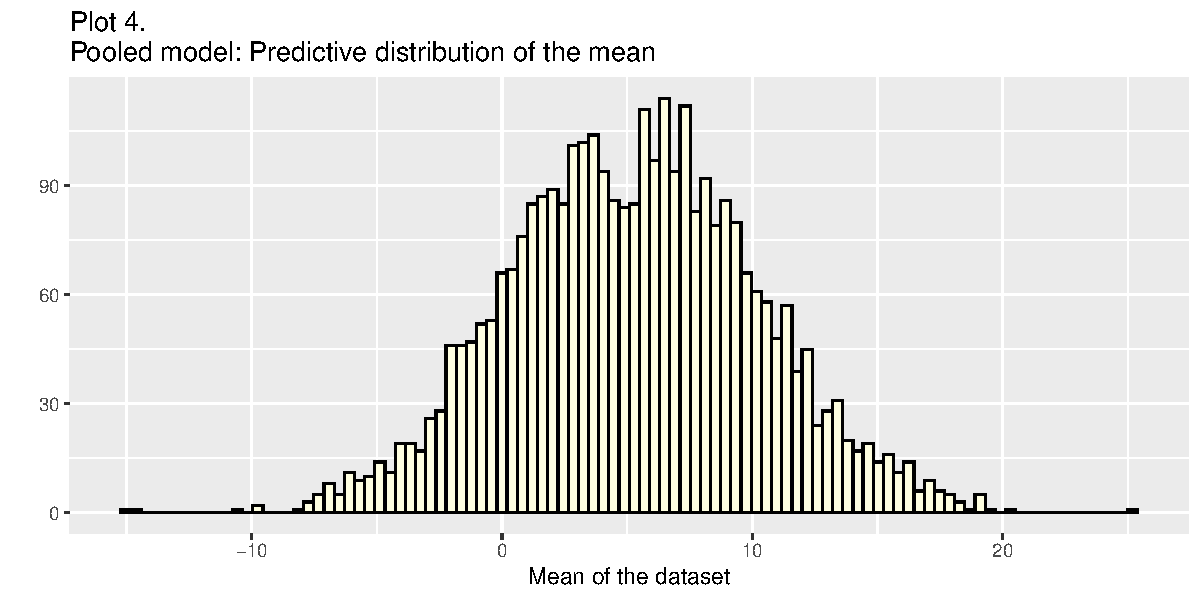
\includegraphics{project_files/figure-latex/fig2-1} \end{center}

\begin{center}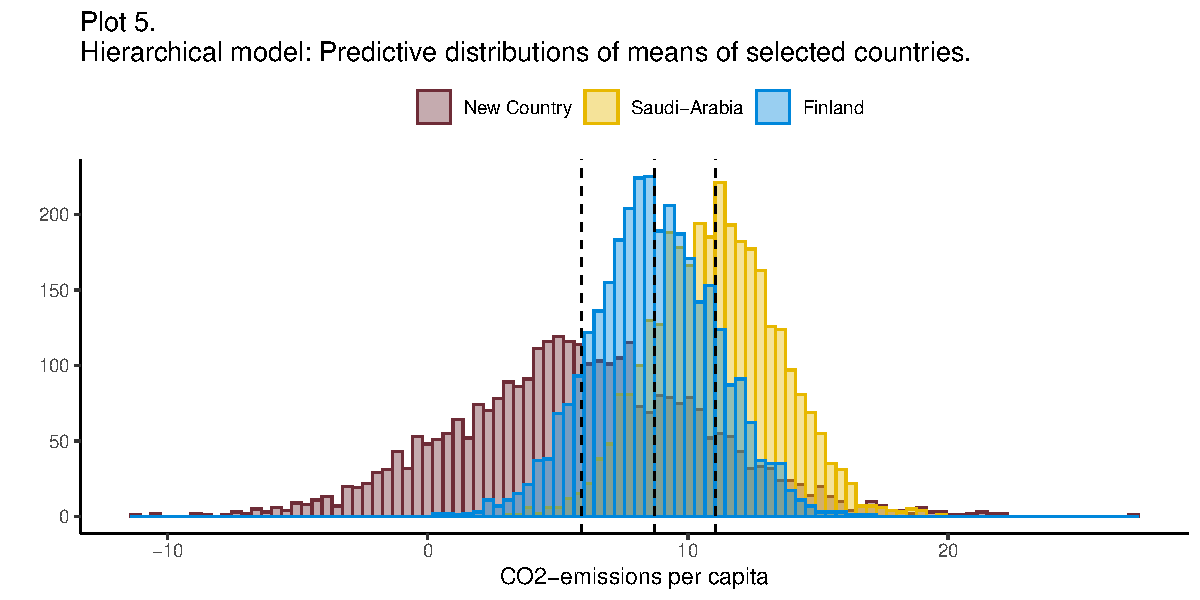
\includegraphics{project_files/figure-latex/fig2-2} \end{center}

\begin{Shaded}
\begin{Highlighting}[]
\NormalTok{mcse\_all \textless{}{-}}\StringTok{ }\NormalTok{bayestestR}\OperatorTok{::}\KeywordTok{mcse}\NormalTok{(hier\_fit)}
\NormalTok{mcse\_new \textless{}{-}}\StringTok{ }\KeywordTok{round}\NormalTok{(mcse\_all}\OperatorTok{$}\NormalTok{MCSE[}\DecValTok{22}\NormalTok{], }\DecValTok{2}\NormalTok{)}
\NormalTok{mcse\_sau \textless{}{-}}\StringTok{ }\KeywordTok{round}\NormalTok{(mcse\_all}\OperatorTok{$}\NormalTok{MCSE[}\DecValTok{23}\NormalTok{], }\DecValTok{2}\NormalTok{)}
\NormalTok{mcse\_fin \textless{}{-}}\StringTok{ }\KeywordTok{round}\NormalTok{(mcse\_all}\OperatorTok{$}\NormalTok{MCSE[}\DecValTok{24}\NormalTok{], }\DecValTok{2}\NormalTok{)}

\NormalTok{mean\_new \textless{}{-}}\StringTok{ }\KeywordTok{round}\NormalTok{(}\KeywordTok{mean}\NormalTok{(hier\_df}\OperatorTok{$}\NormalTok{y\_pred\_new\_county), }\DecValTok{1}\NormalTok{)}
\NormalTok{mean\_sau \textless{}{-}}\StringTok{ }\KeywordTok{round}\NormalTok{(}\KeywordTok{mean}\NormalTok{(hier\_df}\OperatorTok{$}\NormalTok{y\_pred\_SAU), }\DecValTok{1}\NormalTok{)}
\NormalTok{mean\_fin \textless{}{-}}\StringTok{ }\KeywordTok{round}\NormalTok{(}\KeywordTok{mean}\NormalTok{(hier\_df}\OperatorTok{$}\NormalTok{y\_pred\_FIN), }\DecValTok{1}\NormalTok{)}

\NormalTok{msce\_quantile\_new\_low \textless{}{-}}\StringTok{ }\KeywordTok{mcse\_quantile}\NormalTok{(hier\_df}\OperatorTok{$}\NormalTok{y\_pred\_new\_county, }\FloatTok{0.05}\NormalTok{)}\OperatorTok{$}\NormalTok{mcse}
\NormalTok{msce\_quantile\_new\_high \textless{}{-}}\StringTok{ }\KeywordTok{mcse\_quantile}\NormalTok{(hier\_df}\OperatorTok{$}\NormalTok{y\_pred\_new\_county, }\FloatTok{0.95}\NormalTok{)}\OperatorTok{$}\NormalTok{mcse}

\NormalTok{msce\_quantile\_sau\_low \textless{}{-}}\StringTok{ }\KeywordTok{mcse\_quantile}\NormalTok{(hier\_df}\OperatorTok{$}\NormalTok{y\_pred\_SAU, }\FloatTok{0.05}\NormalTok{)}\OperatorTok{$}\NormalTok{mcse}
\NormalTok{msce\_quantile\_sau\_high \textless{}{-}}\StringTok{ }\KeywordTok{mcse\_quantile}\NormalTok{(hier\_df}\OperatorTok{$}\NormalTok{y\_pred\_SAU, }\FloatTok{0.95}\NormalTok{)}\OperatorTok{$}\NormalTok{mcse}

\NormalTok{msce\_quantile\_fin\_low \textless{}{-}}\StringTok{ }\KeywordTok{mcse\_quantile}\NormalTok{(hier\_df}\OperatorTok{$}\NormalTok{y\_pred\_FIN, }\FloatTok{0.05}\NormalTok{)}\OperatorTok{$}\NormalTok{mcse}
\NormalTok{msce\_quantile\_fin\_high \textless{}{-}}\StringTok{ }\KeywordTok{mcse\_quantile}\NormalTok{(hier\_df}\OperatorTok{$}\NormalTok{y\_pred\_FIN, }\FloatTok{0.95}\NormalTok{)}\OperatorTok{$}\NormalTok{mcse}

\NormalTok{quantile\_new \textless{}{-}}\StringTok{ }\KeywordTok{round}\NormalTok{(}\KeywordTok{quantile}\NormalTok{(hier\_df}\OperatorTok{$}\NormalTok{y\_pred\_new\_county, }\KeywordTok{c}\NormalTok{(}\FloatTok{0.05}\NormalTok{, }\FloatTok{0.95}\NormalTok{)), }\DecValTok{0}\NormalTok{)}
\NormalTok{quantile\_sau \textless{}{-}}\StringTok{ }\KeywordTok{round}\NormalTok{(}\KeywordTok{quantile}\NormalTok{(hier\_df}\OperatorTok{$}\NormalTok{y\_pred\_SAU, }\KeywordTok{c}\NormalTok{(}\FloatTok{0.05}\NormalTok{, }\FloatTok{0.95}\NormalTok{)), }\DecValTok{0}\NormalTok{)}
\NormalTok{quantile\_fin \textless{}{-}}\StringTok{ }\KeywordTok{round}\NormalTok{(}\KeywordTok{quantile}\NormalTok{(hier\_df}\OperatorTok{$}\NormalTok{y\_pred\_FIN, }\KeywordTok{c}\NormalTok{(}\FloatTok{0.05}\NormalTok{, }\FloatTok{0.95}\NormalTok{)), }\DecValTok{1}\NormalTok{)}
\end{Highlighting}
\end{Shaded}

The predictive distribution of CO\(_2\) per capita emission of the
Kingdom of Saudi Arabia (SAU) is presented above. The mean of the
predictive distribution is 11.1 with MCSE 0.04\ldots{} A standard
deviation for Saudi-Arabia is 2.4, 5\% quantile 7 and 95\% qauntile 15.
Comparing this to the time-series figure in Section 2, the predicted
value appears to be slightly too small. That's due to the fast increase
in emissions which happened between 1950-1980. Our hierarchical model
also counts values from that time interval, which causes too small
values from the predictive distribution. Otherwise, the shape of the
distribution looks as expected.

The mean of Finland's (FIN) predictive distribution is roughly 9, which
seems to be correct comparing it to the development of previous years
(Section 2 picture). There is also some amount of uncertainty in
distribution, so Q5 is at point 4.7 and Q95 at point 12.6. That's a
moderately conservative distribution, and it's not possible to do
accurate estimates based on this distribution. It still can give an
estimate from which broad conclusions can be drawn about the level of
emissions. For example, if we compare SAU's and FIN's predictive
distribution, the higher level can be deduced, although accurate
estimates could not be made.

Next, let's analyze the prediction distribution of our hierarchical
model for the new country. The first positive sign is that the mean
settled down to about 5.5, which is also the most likely possibility
inferred from the Section 2 figure based on the data used. The moderate
large standard deviation also limits its predictive power for this
forecast variable, but again gives direction, which could be the new
country's emissions level. Usage of the normal gaussian hierarchical
model is causing the distribution to spread to the negative consumption
side, which is an possible downside. We are going to discuss potential
improvements in Section 11. These same considerations also apply to the
sample prediction done from the pooled model.

\hypertarget{model-comparison}{%
\section{9. Model comparison}\label{model-comparison}}

Next, we will present the model comparison between our two models. The
comparison is done with the PSIS-LOO stan package. When doing the
relative EFF calculation from logarithmic likelihood values, the total
number of 4 cores is utilized.

\begin{Shaded}
\begin{Highlighting}[]
\NormalTok{pool\_model\_loglik \textless{}{-}}\StringTok{ }\NormalTok{rstan}\OperatorTok{::}\KeywordTok{stan\_model}\NormalTok{(}\DataTypeTok{file =} \StringTok{"pooled\_model\_stan.stan"}\NormalTok{)}
\end{Highlighting}
\end{Shaded}

\begin{verbatim}
## Running /usr/lib/R/bin/R CMD SHLIB foo.c
## clang -flto=thin -std=gnu99 -I"/usr/share/R/include" -DNDEBUG   -I"/usr/local/lib/R/site-library/Rcpp/include/"  -I"/usr/local/lib/R/site-library/RcppEigen/include/"  -I"/usr/local/lib/R/site-library/RcppEigen/include/unsupported"  -I"/usr/local/lib/R/site-library/BH/include" -I"/usr/local/lib/R/site-library/StanHeaders/include/src/"  -I"/usr/local/lib/R/site-library/StanHeaders/include/"  -I"/usr/local/lib/R/site-library/RcppParallel/include/"  -I"/usr/local/lib/R/site-library/rstan/include" -DEIGEN_NO_DEBUG  -DBOOST_DISABLE_ASSERTS  -DBOOST_PENDING_INTEGER_LOG2_HPP  -DSTAN_THREADS  -DBOOST_NO_AUTO_PTR  -include '/usr/local/lib/R/site-library/StanHeaders/include/stan/math/prim/mat/fun/Eigen.hpp'  -D_REENTRANT -DRCPP_PARALLEL_USE_TBB=1     -fpic  -g -O2 -fdebug-prefix-map=/build/r-base-jbaK_j/r-base-3.6.3=. -fstack-protector-strong -Wformat -Werror=format-security -Wdate-time -D_FORTIFY_SOURCE=2 -g  -c foo.c -o foo.o
## In file included from <built-in>:1:
## In file included from /usr/local/lib/R/site-library/StanHeaders/include/stan/math/prim/mat/fun/Eigen.hpp:13:
## In file included from /usr/local/lib/R/site-library/RcppEigen/include/Eigen/Dense:1:
## In file included from /usr/local/lib/R/site-library/RcppEigen/include/Eigen/Core:88:
## /usr/local/lib/R/site-library/RcppEigen/include/Eigen/src/Core/util/Macros.h:613:1: error: unknown type name 'namespace'
## namespace Eigen {
## ^
## /usr/local/lib/R/site-library/RcppEigen/include/Eigen/src/Core/util/Macros.h:613:16: error: expected ';' after top level declarator
## namespace Eigen {
##                ^
##                ;
## In file included from <built-in>:1:
## In file included from /usr/local/lib/R/site-library/StanHeaders/include/stan/math/prim/mat/fun/Eigen.hpp:13:
## In file included from /usr/local/lib/R/site-library/RcppEigen/include/Eigen/Dense:1:
## /usr/local/lib/R/site-library/RcppEigen/include/Eigen/Core:96:10: fatal error: 'complex' file not found
## #include <complex>
##          ^~~~~~~~~
## 3 errors generated.
## make: *** [/usr/lib/R/etc/Makeconf:168: foo.o] Error 1
\end{verbatim}

\begin{Shaded}
\begin{Highlighting}[]
\NormalTok{pool\_fit\_loglik \textless{}{-}}\StringTok{ }\NormalTok{rstan}\OperatorTok{::}\KeywordTok{sampling}\NormalTok{(}\DataTypeTok{object =}\NormalTok{ pool\_model\_loglik,}
                            \DataTypeTok{data =}\NormalTok{ pool\_data,}
                            \DataTypeTok{iter =}\NormalTok{ num\_of\_iter,}
                            \DataTypeTok{warmup =}\NormalTok{ num\_of\_warmup,}
                            \DataTypeTok{refresh =} \DecValTok{0}\NormalTok{)}

\NormalTok{hier\_model\_loglik \textless{}{-}}\StringTok{ }\NormalTok{rstan}\OperatorTok{::}\KeywordTok{stan\_model}\NormalTok{(}\DataTypeTok{file =} \StringTok{"hierarchical\_model\_stan.stan"}\NormalTok{)}
\end{Highlighting}
\end{Shaded}

\begin{verbatim}
## Running /usr/lib/R/bin/R CMD SHLIB foo.c
## clang -flto=thin -std=gnu99 -I"/usr/share/R/include" -DNDEBUG   -I"/usr/local/lib/R/site-library/Rcpp/include/"  -I"/usr/local/lib/R/site-library/RcppEigen/include/"  -I"/usr/local/lib/R/site-library/RcppEigen/include/unsupported"  -I"/usr/local/lib/R/site-library/BH/include" -I"/usr/local/lib/R/site-library/StanHeaders/include/src/"  -I"/usr/local/lib/R/site-library/StanHeaders/include/"  -I"/usr/local/lib/R/site-library/RcppParallel/include/"  -I"/usr/local/lib/R/site-library/rstan/include" -DEIGEN_NO_DEBUG  -DBOOST_DISABLE_ASSERTS  -DBOOST_PENDING_INTEGER_LOG2_HPP  -DSTAN_THREADS  -DBOOST_NO_AUTO_PTR  -include '/usr/local/lib/R/site-library/StanHeaders/include/stan/math/prim/mat/fun/Eigen.hpp'  -D_REENTRANT -DRCPP_PARALLEL_USE_TBB=1     -fpic  -g -O2 -fdebug-prefix-map=/build/r-base-jbaK_j/r-base-3.6.3=. -fstack-protector-strong -Wformat -Werror=format-security -Wdate-time -D_FORTIFY_SOURCE=2 -g  -c foo.c -o foo.o
## In file included from <built-in>:1:
## In file included from /usr/local/lib/R/site-library/StanHeaders/include/stan/math/prim/mat/fun/Eigen.hpp:13:
## In file included from /usr/local/lib/R/site-library/RcppEigen/include/Eigen/Dense:1:
## In file included from /usr/local/lib/R/site-library/RcppEigen/include/Eigen/Core:88:
## /usr/local/lib/R/site-library/RcppEigen/include/Eigen/src/Core/util/Macros.h:613:1: error: unknown type name 'namespace'
## namespace Eigen {
## ^
## /usr/local/lib/R/site-library/RcppEigen/include/Eigen/src/Core/util/Macros.h:613:16: error: expected ';' after top level declarator
## namespace Eigen {
##                ^
##                ;
## In file included from <built-in>:1:
## In file included from /usr/local/lib/R/site-library/StanHeaders/include/stan/math/prim/mat/fun/Eigen.hpp:13:
## In file included from /usr/local/lib/R/site-library/RcppEigen/include/Eigen/Dense:1:
## /usr/local/lib/R/site-library/RcppEigen/include/Eigen/Core:96:10: fatal error: 'complex' file not found
## #include <complex>
##          ^~~~~~~~~
## 3 errors generated.
## make: *** [/usr/lib/R/etc/Makeconf:168: foo.o] Error 1
\end{verbatim}

\begin{Shaded}
\begin{Highlighting}[]
\NormalTok{hier\_fit\_loglik \textless{}{-}}\StringTok{ }\NormalTok{rstan}\OperatorTok{::}\KeywordTok{sampling}\NormalTok{(}\DataTypeTok{object =}\NormalTok{ hier\_model\_loglik,}
                            \DataTypeTok{data =}\NormalTok{ hier\_data,}
                            \DataTypeTok{iter =}\NormalTok{ num\_of\_iter,}
                            \DataTypeTok{warmup =}\NormalTok{ num\_of\_warmup,}
                            \DataTypeTok{refresh =} \DecValTok{0}\NormalTok{)}
\end{Highlighting}
\end{Shaded}

\begin{Shaded}
\begin{Highlighting}[]
\NormalTok{log\_lik\_pooled \textless{}{-}}\StringTok{ }\KeywordTok{extract\_log\_lik}\NormalTok{(pool\_fit\_loglik, }\DataTypeTok{merge\_chains =} \OtherTok{FALSE}\NormalTok{)}
\NormalTok{r\_eff\_pooled \textless{}{-}}\StringTok{ }\KeywordTok{relative\_eff}\NormalTok{(}\KeywordTok{exp}\NormalTok{(log\_lik\_pooled), }\DataTypeTok{cores=}\DecValTok{4}\NormalTok{)}
\NormalTok{loo\_pooled \textless{}{-}}\StringTok{ }\KeywordTok{loo}\NormalTok{(log\_lik\_pooled, }\DataTypeTok{r\_eff =}\NormalTok{ r\_eff\_pooled, }\DataTypeTok{cores =} \DecValTok{4}\NormalTok{)}
\KeywordTok{print}\NormalTok{(loo\_pooled)}
\end{Highlighting}
\end{Shaded}

\begin{verbatim}
## 
## Computed from 3200 by 1311 log-likelihood matrix
## 
##          Estimate   SE
## elpd_loo  -3993.8 32.2
## p_loo         2.5  0.2
## looic      7987.6 64.5
## ------
## Monte Carlo SE of elpd_loo is 0.0.
## 
## All Pareto k estimates are good (k < 0.5).
## See help('pareto-k-diagnostic') for details.
\end{verbatim}

\begin{Shaded}
\begin{Highlighting}[]
\NormalTok{log\_lik\_hier \textless{}{-}}\StringTok{ }\KeywordTok{extract\_log\_lik}\NormalTok{(hier\_fit\_loglik, }\DataTypeTok{merge\_chains =} \OtherTok{FALSE}\NormalTok{)}
\NormalTok{r\_eff\_hier \textless{}{-}}\StringTok{ }\KeywordTok{relative\_eff}\NormalTok{(}\KeywordTok{exp}\NormalTok{(log\_lik\_hier), }\DataTypeTok{cores=}\DecValTok{4}\NormalTok{)}
\NormalTok{loo\_hier \textless{}{-}}\StringTok{ }\KeywordTok{loo}\NormalTok{(log\_lik\_hier, }\DataTypeTok{r\_eff =}\NormalTok{ r\_eff\_pooled, }\DataTypeTok{cores =} \DecValTok{4}\NormalTok{)}
\KeywordTok{print}\NormalTok{(loo\_hier)}
\end{Highlighting}
\end{Shaded}

\begin{verbatim}
## 
## Computed from 3200 by 1311 log-likelihood matrix
## 
##          Estimate   SE
## elpd_loo  -3014.2 48.1
## p_loo        21.6  1.8
## looic      6028.4 96.3
## ------
## Monte Carlo SE of elpd_loo is 0.1.
## 
## All Pareto k estimates are good (k < 0.5).
## See help('pareto-k-diagnostic') for details.
\end{verbatim}

\begin{Shaded}
\begin{Highlighting}[]
\KeywordTok{plot}\NormalTok{(loo\_pooled,}
\DataTypeTok{diagnostic=}\KeywordTok{c}\NormalTok{(}\StringTok{"k"}\NormalTok{, }\StringTok{"n\_eff"}\NormalTok{),}
\DataTypeTok{main=}\StringTok{"PSIS reliability diagnostics for pooled model"}\NormalTok{)}
\end{Highlighting}
\end{Shaded}

\includegraphics{project_files/figure-latex/unnamed-chunk-11-1.pdf}

\begin{Shaded}
\begin{Highlighting}[]
\KeywordTok{plot}\NormalTok{(loo\_hier,}
\DataTypeTok{diagnostic=}\KeywordTok{c}\NormalTok{(}\StringTok{"k"}\NormalTok{, }\StringTok{"n\_eff"}\NormalTok{),}
\DataTypeTok{main=}\StringTok{"PSIS reliability diagnostics for hierarchical model"}\NormalTok{)}
\end{Highlighting}
\end{Shaded}

\includegraphics{project_files/figure-latex/unnamed-chunk-11-2.pdf} When
inspecting the comparison plots, the first clear observation is that all
Pareto k diagnostic values are between \(\infty\) and 0.5, so the
PSIS-LOO -values of both models can be considered reliable. The values
over 0.5 start to be problematic, which could lead to the need to
re-evaluate the model, but in our case, the values are all low enough.
Next, it is important to check how large p\_loo is compared to the
number of parameters of the model. In general, if p\_loo is less than or
approximately equal to the number of model parameters, the model can be
considered well specified. The number of parameters of the pooled model
is 2 when its p\_loo is 2.5. Thus, the percentage of parameters is
exceeded by 25\%. Respectively, the number of parameters of the
hierarchical model is 22, when its p\_loo value is 22.4. Thus, the
percentage of parameters is exceeded by 0.9\%. The p\_loo value shows
that the hierarchical model's performance seems more reasonable when
considered the problem in-hand.

The last PSIS-LOO's comparison variable, which we are going to inspect,
is an elpd\_loo. The less negative the value of elpd\_loo is, the better
the fit of the model to that problem can be considered to be. The values
of elpd\_loo are presented above. Now, it's easy starting to be easy to
deduce that the hierarchical model is a better fit for this problem. Its
elpd\_loo value is over 900 higher than the corresponding value of the
pooled model.

\hypertarget{sensitivity-analysis-priors}{%
\section{10. Sensitivity analysis
(Priors)}\label{sensitivity-analysis-priors}}

In this part, we'll examine the effect of priors to the predictive
distribution of Finland and a country outside our dataset (namely new
country) with hierarchical model. We'll use three different priors and
plot the end results to easily-comparable histograms to see if there is
a lot of variation.

\hypertarget{choosing-differing-priors}{%
\subsection{10.1 Choosing differing
priors}\label{choosing-differing-priors}}

As a reminder, we decided to use following values to model hyper mu,
hyper sigma and common sigma: hyper\_mu \(\sim\) lNorm(2.58, 0.5)
hyper\_sigma \(\sim\) Gamma(2.5, 0.8) sigma \(\sim\)
inv\_chi\_square(2.5)

Next, under the hood, we'll do the same modeling but with different
priors. The actual code is printed in the appendix. Please note that we
had to change the value of warm-ups from 200 to 400 as there started to
appear divergent transitions with in the tests.

Our idea is to see what happens if we relax our priors a lot, and on the
contrary, what happens if we make them tighter. We'll use the following
values for the listed models:

Relaxed model: hyper\_mu \(\sim\) lNorm(5.0, 0.5) hyper\_sigma \(\sim\)
Gamma(2, 50) sigma \(\sim\) inv\_chi\_square(0.1)

Tightened model: hyper\_mu \(\sim\) lNorm(0.01, 1) hyper\_sigma \(\sim\)
Gamma(1.1, 0.6) sigma \(\sim\) inv\_chi\_square(10)

\hypertarget{plotting-the-results}{%
\subsection{10.2 Plotting the results}\label{plotting-the-results}}

\begin{verbatim}
## Warning: There were 11 divergent transitions after warmup. See
## http://mc-stan.org/misc/warnings.html#divergent-transitions-after-warmup
## to find out why this is a problem and how to eliminate them.
\end{verbatim}

\begin{verbatim}
## Warning: Examine the pairs() plot to diagnose sampling problems
\end{verbatim}

\begin{center}\includegraphics{project_files/figure-latex/fig3-1} \end{center}

\hypertarget{issues-and-potential-improvements}{%
\section{11. Issues and potential
improvements}\label{issues-and-potential-improvements}}

In this section, we are going to list possible issues related to, for
example, the used models. From the problems, we get directly to possible
development ideas that could be interesting to implement in the future.
The first potential issue is related to data reliability, which always
has to be taken into consideration when data from open-source is used.
In the worst case, the use of manipulated data can lead to significantly
detrimental conclusions, for example, when considering policy
recommendations. At the beginning of the work, we looked at the source
of the data from many different angles, which makes it seem unlikely
that the data storers had modified it. A greater concern is the
reliability of samples from different countries. For example, it may be
in the interests of some parties to beautify the country's CO2
emissions, making the data unreliable. This potential issue should be
kept in mind when looking at the results.

Another issue arose at the prediction stage when the probability
distribution provided the possibility to get values below zero, which
depending on the definition, either does not make sense or means the
removal of CO\(_2\) emissions from the atmosphere (carbon negativity).
If we choose carbon negativity as the definition of negative values, the
distribution is too broad (too high a probability for carbon negativity)
but otherwise possible. If, on the other hand, we think that emissions
cannot be negative (as in the choice of a priori), the tail is a real
issue. The possible improvement is to use some other hierarchical model
than Gaussian when modeling this phenomenon. Using a different
hierarchical model could be an excellent experimental topic for further
development of the work.

As mentioned above, the one possible improvement is to use a different
hierarchical model to the same dataset (one possibility could be, for
example, a lognormal model). One could also divide countries into
different sets based on different geographical locations and use these
as groups in a hierarchical model. The division could also be made based
on some other characteristic, in which case different conclusions could
also be drawn from the results. The observation period can also be
changed, and its effect on averages and forecasts monitored. One
development idea that would require a little more know-how from the
implementer would be to study the effect of CO2 emissions on temperature
and use the results of the work to predict temperature development in
different regions. An implementation of the same style, but which is
taken further, is shown in Figure \ref{fig:annual_global_emission}.
Figure \ref{fig:annual_global_emission} shows the effect of various
policy recommendations on emissions and thus on temperature.

\begin{figure}
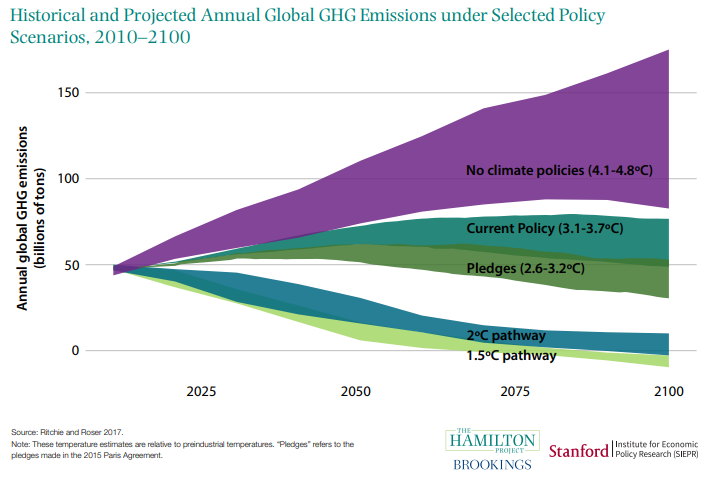
\includegraphics[width=1\linewidth]{annual_global_emission} \caption{\label{fig:annual_global_emission}Annual global emissions -- }\label{fig:annual_global_emiss}
\end{figure}

\hypertarget{what-was-learned}{%
\section{12. What was learned}\label{what-was-learned}}

\hypertarget{self-reflection}{%
\section{13. Self-reflection}\label{self-reflection}}

\begin{Shaded}
\begin{Highlighting}[]
\NormalTok{pooled\_plotters \textless{}{-}}\StringTok{ }\ControlFlowTok{function}\NormalTok{() \{}
\NormalTok{  pooled\_df =}\KeywordTok{data.frame}\NormalTok{(rstan}\OperatorTok{::}\KeywordTok{extract}\NormalTok{(pool\_fit, }\DataTypeTok{permuted=}\NormalTok{T))}
  
  \CommentTok{\#Histogram}
  \KeywordTok{hist}\NormalTok{(pooled\_df}\OperatorTok{$}\NormalTok{mu, }
       \DataTypeTok{breaks =} \DecValTok{100}\NormalTok{,}
       \DataTypeTok{xlim=}\KeywordTok{c}\NormalTok{(}\DecValTok{0}\NormalTok{,}\DecValTok{22}\NormalTok{),}
       \DataTypeTok{xlab =} \StringTok{"Mean of the quality measurements"}\NormalTok{,}
       \DataTypeTok{col =} \StringTok{"lightyellow"}\NormalTok{,}
       \DataTypeTok{main=}\StringTok{"Posterior distribution of the mean of the sixth machine"}\NormalTok{)}
\NormalTok{\}}
\end{Highlighting}
\end{Shaded}

\begin{Shaded}
\begin{Highlighting}[]
\NormalTok{hierarchical\_plotters \textless{}{-}}\StringTok{ }\ControlFlowTok{function}\NormalTok{() \{}
\NormalTok{  hierarchical\_df =}\KeywordTok{data.frame}\NormalTok{(rstan}\OperatorTok{::}\KeywordTok{extract}\NormalTok{(hier\_fit, }\DataTypeTok{permuted=}\NormalTok{T))}
  
  \CommentTok{\#MCMC Areas}
\NormalTok{  mcmc\_areas\_df \textless{}{-}}\StringTok{ }\NormalTok{hierarchical\_df }\OperatorTok{\%\textgreater{}\%}\StringTok{ }\KeywordTok{select}\NormalTok{(}\KeywordTok{starts\_with}\NormalTok{(}\StringTok{\textquotesingle{}mu\textquotesingle{}}\NormalTok{)) }\OperatorTok{\%\textgreater{}\%}
\StringTok{                    }\KeywordTok{setNames}\NormalTok{(}\KeywordTok{colnames}\NormalTok{(data\_co2\_population))}
  \KeywordTok{mcmc\_areas}\NormalTok{(mcmc\_areas\_df) }\OperatorTok{+}\StringTok{ }\KeywordTok{xlab}\NormalTok{(}\StringTok{"Testttttttt"}\NormalTok{)}
  
  \CommentTok{\#Histograms of countries together}
\NormalTok{  m \textless{}{-}}\StringTok{ }\DecValTok{19}
\NormalTok{  \{}
  \KeywordTok{plot}\NormalTok{(}\DecValTok{0}\NormalTok{,}\DecValTok{0}\NormalTok{,}\DataTypeTok{type=}\StringTok{"n"}\NormalTok{,}
        \DataTypeTok{xlim=}\KeywordTok{c}\NormalTok{(}\DecValTok{0}\NormalTok{,}\DecValTok{20}\NormalTok{), }\DataTypeTok{ylim=}\KeywordTok{c}\NormalTok{(}\DecValTok{0}\NormalTok{,}\DecValTok{1100}\NormalTok{),}
        \DataTypeTok{xlab=}\StringTok{"x"}\NormalTok{,}\DataTypeTok{ylab=}\StringTok{"freq"}\NormalTok{, }
        \DataTypeTok{main=}\StringTok{"Histograms of each country separately, plotted together"}\NormalTok{)}
    \ControlFlowTok{for}\NormalTok{(n }\ControlFlowTok{in} \DecValTok{1}\OperatorTok{:}\NormalTok{m) \{}
\NormalTok{      var\_name \textless{}{-}}\StringTok{ }\KeywordTok{paste}\NormalTok{(}\StringTok{"mu."}\NormalTok{,n, }\DataTypeTok{sep=}\StringTok{""}\NormalTok{)}
      \CommentTok{\#hier\_matrix[n,] \textless{}{-} unlist(hierarchical\_df[var\_name])}
      \KeywordTok{plot}\NormalTok{(}
        \KeywordTok{hist}\NormalTok{(}\KeywordTok{unlist}\NormalTok{(hierarchical\_df[var\_name]), }\DataTypeTok{breaks =} \DecValTok{12}\NormalTok{, }\DataTypeTok{plot=}\OtherTok{FALSE}\NormalTok{),}
        \DataTypeTok{col=}\KeywordTok{alpha}\NormalTok{(}\StringTok{\textquotesingle{}blue\textquotesingle{}}\NormalTok{, }\FloatTok{0.25}\NormalTok{),}
        \DataTypeTok{add=}\NormalTok{T }\CommentTok{\# Add to main plot}
\NormalTok{        )  }
\NormalTok{    \}}
\NormalTok{  \}}
  
  \CommentTok{\#One histogram for whole data}
\NormalTok{  one\_hist\_data \textless{}{-}}\StringTok{ }\KeywordTok{unlist}\NormalTok{(hierarchical\_df }\OperatorTok{\%\textgreater{}\%}\StringTok{ }\KeywordTok{select}\NormalTok{(}\KeywordTok{starts\_with}\NormalTok{(}\StringTok{\textquotesingle{}mu\textquotesingle{}}\NormalTok{)))}
  \KeywordTok{plot}\NormalTok{(}\KeywordTok{hist}\NormalTok{(one\_hist\_data, }\DataTypeTok{breaks =} \DecValTok{100}\NormalTok{, }\DataTypeTok{xlim =} \KeywordTok{c}\NormalTok{(}\DecValTok{0}\NormalTok{,}\DecValTok{22}\NormalTok{), }\DataTypeTok{ylim =} \KeywordTok{c}\NormalTok{(}\DecValTok{0}\NormalTok{, }\DecValTok{5000}\NormalTok{)),}
            \DataTypeTok{col =} \StringTok{\textquotesingle{}lightblue\textquotesingle{}}\NormalTok{)}

\NormalTok{\}}
\end{Highlighting}
\end{Shaded}


\end{document}
